% !TEX program = xelatex

\documentclass[10pt,landscape]{article}
\usepackage{amssymb,amsmath,amsthm,amsfonts}
\usepackage{multicol,multirow}
\usepackage{calc}
\usepackage{ifthen}
\usepackage{graphicx}
\usepackage[landscape]{geometry}
\usepackage[colorlinks=true,citecolor=blue,linkcolor=blue]{hyperref}
\usepackage{polyglossia}
\setdefaultlanguage{english}
\setotherlanguages{farsi}
\newfontfamily\arabicfont{XB Niloofar}
\graphicspath{ {./} }
\ifthenelse{\lengthtest { \paperwidth = 11in}}
    { \geometry{top=.5in,left=.5in,right=.5in,bottom=.5in} }
	{\ifthenelse{ \lengthtest{ \paperwidth = 297mm}}
		{\geometry{top=1cm,left=1cm,right=1cm,bottom=1cm} }
		{\geometry{top=1cm,left=1cm,right=1cm,bottom=1cm} }
	}
\pagestyle{empty}
\makeatletter
\renewcommand{\section}{\@startsection{section}{1}{0mm}%
                                {-1ex plus -.5ex minus -.2ex}%
                                {0.5ex plus .2ex}%x
                                {\normalfont\large\bfseries}}
\renewcommand{\subsection}{\@startsection{subsection}{2}{0mm}%
                                {-1explus -.5ex minus -.2ex}%
                                {0.5ex plus .2ex}%
                                {\normalfont\normalsize\bfseries}}
\renewcommand{\subsubsection}{\@startsection{subsubsection}{3}{0mm}%
                                {-1ex plus -.5ex minus -.2ex}%
                                {1ex plus .2ex}%
                                {\normalfont\small\bfseries}}
\makeatother
\setcounter{secnumdepth}{0}
\setlength{\parindent}{0pt}
\setlength{\parskip}{0pt plus 0.5ex}
% -----------------------------------------------------------------------

\title{Quick Guide to LaTeX}

\begin{document}

\raggedright
\footnotesize

\begin{center}
     \Large{\textbf{Scientific and Technical Presentation Cheat Sheet}} \\
\end{center}
\begin{multicols*}{3}
\setlength{\premulticols}{1pt}
\setlength{\postmulticols}{1pt}
\setlength{\multicolsep}{1pt}
\setlength{\columnsep}{2pt}

%
\section{Reasons of Scientific Presentation}
engineers present a lot(40\%) |
engineers require strong presentation skills , strong social skills |
iranians are weak (reporting , presentation , social skills)| unethical not to publish |
results worth presenting |
progressing scientific thought |
credibility | broad receiver |
promotion | research grants 

\section{Order of Learning}
Reading(10\%) Hearing(20\%) Seeing(30\%)
Seeing \& Hearing(50\%) Discussing(70\%) 
Experimenting(80\%) Teaching(95\%)

\section{Communication}
No radio talk |
7\% Words 38\% Voice tone 55\% body language 

\section{Research Procedure}
rough outline: Ideation, Background Preparation, Topic Selection, 
Initial Research \& Proposal Development, Proposal Defense,
Research Completion, Thesis Defense, Publication

Ideation: understand topic, its importance \& related issues

Background Preparation: find key conferences \& journals, key authors \& distinguished researcher labs

Topic Selection: know the topics, main issues \& like it

Initial Research \& Proposal Development: fundamental activity, Study most relevant aspects,
put adequate time \& attention, Understand the project, make a plan, carry out plan, look back on your work 

How to Select paper: 3\-pass approach (1st pass gives general idea , 2nd pass grasp papers content, 3rd pass in depth)

1st pass: bird's-eye view, 1. 5-10min read title, abstract \& introduction, 2. read subsection headings ignore everything else
3. Read conclusion, 4. Glance over the references 
after 1st pass you should know 5C's(Category, Context, Correctness, Contributions, Clarity)

2nd pass: about 1 hour , 1. look carefully at illustrations \& pay attention to graphs
2. mark relevant unread references

3rd pass: about 4-5 hours for beginners (1 hour for experts), The key is to attempt to virtually reimplement it
,This pass requires a great attention to detail

Literature Survey:
First, use an academic search engine to
find 3-5 recent papers in the area. If you can find a survey paper, you are done
Second, find shared citations \& repeated authors in
the bibliography Third, go to the website for these top conferences \&
look through their recent proceedings

Literature Review Ordering: Text Books, Ph.D Dissertations, Survey Articles, Journal Papers,
Conference Papers, Technical Reports, Research Lab \& Internet Sites, Scientific Seminars

Finding good review/survey is extremely useful

Print important papers to read | keep track of all articles

Publication: publication is the end result of work into research |
publish or perish syndrome 

\section{Scientific \& Technical Writing}
Writing Stages: 1. Subject Matter 2.Writing Constraints 3.Purpose of Writing 4.Writing Style

first analyze your constraints (Audience, Ocasion, Purpose)

1.Getting in the mood 2.Writing the first Draft 3.Revising, Revising, Revising 4.Finishing

Main Aspects of Writing: Content, Style(way you communicate), Form

Style: Many journal articles follow a set of organization sections (Introduction, Literature Review, 
Proposed Method, Experimental Results, Conclusion) Beginning: (Title, Abstract, Introduction)

Abstract tells reader what happens in the document. has descriptive or informative approach
abstract clarifies the work.

Introduction: prepares reader for the content. why the research is important.

In the middle of a report you present your work. Choose a logical strategy.
Manage logical sections \& subsections. Section headings should be descriptive \& parallel.
pieces should be of the same pie.

Strategies for middles of Scientific reports: 1.Chronological 2.Spatial 3.Parallel parts
4.Flow

Ending: analyze results \& give future perspective. Analyze with a fair perspective

Ending Ordering: Conclustion, Future Perspective, References, Appendices.
Failing to cite others is a fatal flaw. Detailed derivations in appendices. Codes, Tables \& figures, list of acronyms, glossary, list of symbols, extra info in appendices

Illustration: tables, figures(graphs(line chart, bar chart, pie chart, area chart), images(photo, drawing, diagrams)) 

tables can present words as well as numbers. when presenting numerical data choose between tables \& graphs.
advantage of photograph is realism. advantage of drawing is control of detail.
advantage of diagram is the ability to show flow of a variable through a system.

Language ordering: Precise, Clear, Forthright, Familiar, Concise, Fluid.
no complex words or sentences. stacking adjectives swallows the idea. ambiguity is bad.
don't use weak verbs.try using varying sentence openers.
gunning fog index $F_i = 0.4 ((\frac{N_w}{N_s})+P_{lw})$ where $N_w=$ number of words in typical paragraph
$N_s=$ number of sentences in the paragraph $P_{lw}=$ percentage of long words in the paragraph.
desired gunning fog index is between 10 and 12.

Form: Format(Typography, Layout), Mechanics(Usage, Spelling, Grammar).
Format is the arrangement of type on the page choose a type size that is easy to read.
Mechanics is the application of rules such as grammar, spelling, punctuation \& usage to the act
of writing.

use numbers for more than $10$ quantities.
use numerals for large numbers, decimals, monetary figures. 
for counting, informal measurements, first word of sentence, fewer than $10$, approximations write out numbers.

i.e is latin for id est meaning "that is". e.g. is latin for exempli gratia meaning "for example".
et al. is latin for et alia, meaning "and others".

First time a symbol used, explain it.
Avoid writing french words with persian alphabets.

Comma separates details in a sentence.Two commas represent parantheses.
Colon introduces a formal list.Semi-colon joins two independent clauses.
Most important aspect of grammar understanding what sentence is.

\section{Scientific Manuscript}
Structure: Title, Authorship, Abstract, Keywords, Introduction, Related Work, Proposed Method,
Experimental Results, (Figures, Tables, Equations), Conclusion, Acknowledgement, Appendix, References

Title: orient the work, be precise, get to the point, include main words, less than 15 words
, uppercase \& boldface, no (colon, sign, citation, footnote, equation)

Authorship: who did the work, institutions, address(email)

Abstract: Summary of the paper (about 150 $\sim$ 300 words),
including brief description, its importance, related existing work \& main shortcomings, main
proposed solutions.No (abbreviations, cited references, displayed equations).Mostly one paragraph.

Keywords: selected for computerized search.Conatins about (4 $\sim$ 6) words

Introduction: defines the scope \& pros \& cons of the work.
Contains problem definition, its scientific importance, historical background, relevance to other areas,
your main ideas, assumptions \& limitations, your main contributions, quantified superiorities.
Properly describe \& reference the related work. Give your description about other algorithms.
Last paragraph summary of the paper structure.

Related Works: Describe more related papers and their pros \& cons.

Proposed Method: Describe proposed solution, highlight contributions, state the model assumption \& limitations
, use block diagram \& flowcharts.

Experimental Results: Give complete performance analysis, State the used machine \& language type,
State resource characteristics(size, resolution, etc.), Use figures, tables \& graphs.
Chosen parameter values should make sense. Show the average values \& confidential intervals.

Figures: Put figures immediately after where they are cited. Large figures in one column.
Some space above \& below each figure. Should be self content. All symbols in legend.
Captions appear below \& end with a full stop. Figure numbers no parantheses.
Don't copy images \& No blurry figures.

Tables rules are sort of same as figures.
table units described.

Equation: end with a full stop. Number equations consequently with the number flushed right \&
enclosed in parantheses.

Conclusion: Summarizes what you have done, main ideas, difficulties, conclude based on obtained results.
Include future research direction, Preferably in one paragraph.

Acknowledgement: Comes before appendix. Should be unnumbered. Funding information may also be included.

Appendix: contains material deemed inessential to understanding but included for 
completeness, detailed mathematical proofs, referable tables, glossaries, abbreviations list \& pseudo codes.

References: Use more readily available papers. Follow standard bibliography format.
All references should be cited in the text.

\section{Manuscript Submission}
Ordering: Originality, Submission, Acknowledgement, Copyright, Camera Ready Submission.

Originality: Manuscript should present the research originally performed by the authors.

Submission: submission is mostly done electronically in .pdf, .doc or .ps.
Cover letter of the manuscript should include title, full name of author, list of authors,
short statement of precise problem, major contributions, copyright \& ethic issues.
To use Sharif affiliation, at least one of the authors should be faculty member.
Students are allowed to publish but not under the name of Sharif. 

Acknowledgement: Editor-in-Chief will acknowledgement the receipt of the submitted manuscript.

Copyright: for accepted manuscript, the authors are assumed to have the copyright transferred to 
the publisher.

Camera Ready Submission: The camera version(final version) should follow the style file provided
by the publisher.

\section{Business Correspondence}
Outline: Layout, Format, Occasion.

Layout: Letterhead, Dateline, Inside Address, Reference Line, Salutation, Subject Line, 
Body, Complimentary Close, Company Signature, Signer's identification, Enclosure Reminder, "CC" Notation.

\section{Scientific \& Technical Oral Presenation}
Ordering: Introduction, Three Stylistic Perspectives, Oral Presentation Points, Thesis Defense Webinar.

Introduction: Oral presentation has advantages over documentation. Presenter
can read audience \& react. Presenter receives instant reaction.
Speaker has limited chance to catch errors. Audience cannot look up background material.
Analyze audience.

Effective Conversation: about 75\% of awake time is spent on social contacts.
Better social life, more successful \& happier life.
Improve self-esteem. Respect people. Be open \& interested about other people's thoughts.
Don't underestimate people. People can be amazing. No one is 100\% right.
Chose proper tone. Be open to criticism.

Structure \& Speech:
As with documents oral presenations should have clear beginnings, middles \& ends.
First minute introduce yourself \& your topic.
Beginning prepares audience for work to be presented.
Middle presents the work in logical order.
Ending summarizes main points.

Visual Aids: Presentation slides. Chose easy to read formats. Color can distinguish a Presentation.
Avoid using red, orange. Slides should have organization.

Central to an effective oral is a design that takes into account need of audience.
Organize slides as precise \& logical as possible.
Start with an "Outline" slide.
Make sure visual aids are readable.
Use color to highlight important points.
Don't put too many ideas on one slide.
Explain everything in slide.
Don't put too much math.
Bring enough math to show your point.
Bring backup.
do two rehearsals before the presentation.
Formal dress.
Get audience to focus. Eye contact is important.

Thesis Defense: audiences are expert referees.
Highlight your work \& try to convince them. Discuss pros \& cons of the state-of-the-art relevent 
literature. Be fair evaluating others work.
Have contributions slide.
List future direction.

Webinar: Make sure your room is lit well.

\raggedleft

\section{\textfarsi{نکات فارسی اسلاید‌ها}}
\textfarsi{

    از توسط استفاده نشود. زمان افعال هماهنگ باشد. عدد ترتیبی به صورت حرف.
    ساعت و دقیقه و شماره قرن هر دو صورت.
    عدد آغاز جمله حرف.
    شماره صفحه و جلد و نمودار و نقشه و نظایر به صورت عدد.
    تاریخ تولد و وفات، سال‌های آغاز و پایان حکومت یا وزارت به صورت عدد.
    درصد به صورت عدد. شماره پانوشت به صورت عدد.
    هوا ابری هست
    $\leftarrow$
    هوا ابری است.
    اگرچه
    $\leftarrow$
    هرچه.
    درحال انجام
    $\leftarrow$
    در حال اجرا.
    با این وجود
    $\leftarrow$
    با وجود این.
    عنوان نماینده
    $\leftarrow$
    نمایندگی از.
    پایه‌های دانشگاه را تشکیل می‌دهند
    $\leftarrow$
    پایه‌های دانشگاه‌اند.
    جهت فلان
    $\leftarrow$
    برای فلان.
    مورد تشویق قرار گرفت
    $\leftarrow$
    تشویق شد.
    عدم استفاده نشود.
    می‌باشد
    $\leftarrow$
    است یا هست.
    یک روش
    $\leftarrow$
    روشی.

    اجزای نامه اداری:
    سرلوحه نامه.
    عنوان گیرنده.
    عنوان فرستنده.
    موضوع نامه.
    متن نامه.
    امضا نامه.
    گیرنده رونوشت نامه.

    سرلوحه نامه:
    بالای کاغذ اداری. نام سازمان سمت راست.
    شماره، تاریخ و پیوست سمت چپ.

    عنوان گیرنده:
    شخص، مقام سازمانی و یا واحد سازمانی گیرنده.
    با "به" مشخص شود.

    عنوان فرستنده:
    شخص، مقام سازمانی و یا واحد سازمانی فرستنده.
    با "از" مشخص شود.

    موضوع نامه:
    عبارت کوتاه و گویا.
    با "موضوع" مشخص شود.

    متن نامه:
    مقدمه، اصل پیام، اختتام.

    امضا نامه:
    نام و نام‌خوانوادگی، سمت سازمانی، علامت امضا.
    ارسال بدون امضا بی‌احترامی است.

    گیرندگان رونوشت:
    ذکر رونوشت به. ذکر به ترتیب اهمیت کاری.
    دلیل دریافت رونوشت.

    اندازه و ابعاد نامه:
    A3
    برای نمودارها و صورت‌های مالی.
    A4
    برای نامه‌های با بیش از 5 سطر.
    A5
    برای نامه‌های کمتر از 5 سطر.
    A6
    بدون سرلوحه. برای مبادله‌ی پیام اداری بین کارمندان و یا یادداشت اداری.
}

\section{\textfarsi{نکات فرهنگستان}}
\textfarsi{

    خطاهای مصداقی:

    خطاها و کاربردهای مکروه زبانی:
    به آنچه که
    $\leftarrow$
    به آنچه.
    هوا ابری هست
    $\leftarrow$
    هوا ابری است.
    از سوی
    ،
    به توسط
    ،
    به وسیله‌ی
    استفاده نشود.
    اقبال استفاده نشود.
    اگرچه
    $\leftarrow$
    هرچند.
    اما استفاده نشود.
    درحال انجام
    $\leftarrow$
    در دست اجرا.
    با این وجود
    $\leftarrow$
    با وجود این.
    از اهمیت ویژه برخوردار است
    $\leftarrow$
    اهمیت خاصی دارد.
    به خود اختصاص دادن استفاده نشود.
    به عنوان نماینده
    $\leftarrow$
    به نمایندگی.
    توسط استفاده نشود.
    تسلیت‌باد یا تهنیت‌باد غلط.
    جای‌جای
    $\leftarrow$
    سرتاسر.
    جهت
    $\leftarrow$
    برای.
    جایگزین
    $\leftarrow$
    جانشین.
    حرف اول را زدن استفاده نشود.
    صدای مرا دارید
    $\leftarrow$
    صدای مرا می‌شنوید.
    در ارتباط با استفاده نشود.
    دست اندرکاران
    ،
    دنبال‌کردن استفاده نشود.
    را اضافی حذف شود.
    تا به اینجا نتیجه‌ای را نگرفتیم
    $\leftarrow$
    تا به اینجا نتیجه‌ای نگرفتیم.
    شامل و مشمول به جای هم استفاده نشود.
    طیف 
    $\leftarrow$
    انواع.
    عدم
    $\leftarrow$
    فقدان.
    غیرپخته 
    $\leftarrow$
    ناپخته.
    غیرقابل استفاده نشود.
    مبتلا به آن
    $\leftarrow$
    به آن مبتلا.
    معرف حضورتان
    $\leftarrow$
    معروف حضورتان.
    من بسیار متعجب هستم که
    $\leftarrow$
    بسیار متعجبم که.
    مورد تشویق قرار گرفتند
    $\leftarrow$
    تشویق شدند.
    از نقطه‌نظر هنری
    $\leftarrow$
    از نظر هنری.

    خطاهای نوعی:

    کاربرد فعل.
    حذف بی‌قرینه‌ی
    فعل کمکی.
    دوری اجزای فعل مرکب.
    کاربرد فعل لازم به جای متعدی.
    کاربرد صیغه‌ی مجهول فعل با ذکر عامل.
    رعایت نکردن قواعد فعل و فاعل.
    تغییر شخص.
    ناهم‌اهنگی افعال.
    کاربرد نابه‌جای وجه وصفی.
    اختیار صیغه‌ی فعل به قاعده‌ی زبان مبدا در ترجمه.
    فعل نامناسب.
    فعل بسیط یا فعل مرکب.
    کاربرد حرف اضافه‌ی نامناسب،
    حذف حرف اضافه.
    تعبیرهای نامناسب.
    صفت یا نسبت نامناسب.
    واژه‌ی بیگانه.
    حشو و تکرار.
    آوردن جمله‌ی صله.
    جمله‌ی بسیط دراز.
    شواهد تعقید.


    نشانه‌ها:
    نقطه،
    نشانه‌ی پرسش،
    نشانه‌ی تعجب،
    ویرگول،
    نقطه ویرگول،
    دو نقطه،
    نشانه‌ی تعلیق،
    نشانه‌ی نقل قول،
    خط.

    نقطه:
    در پایان جمله‌ی خبری یا انشایی.
    در مختصرنویسی اسامی و عناوین.

    نشانه‌ی پرسشی:
    پس از جمله‌ی پرسشی.
    برای افاده‌ی حدس و گمان و تردید.

    نشانه‌ی تعجب:
    پس از اصوات.
    در پایان جمله‌ی تعجبی.
    تحذیر یا امر تاکیدی.

    ویرگول:
    پس از منادا.
    برای عطف سازه‌های هم‌پایه.
    پس از گروه قیدی
    (در آغاز جمله)
    و پیش و پس از آن
    (در میان جمله).
    برای مجزا کردن بدل از کل.
    برای مجزا کردن عبارت معترضه‌ی دعایی.
    برای مجزا کردن عبارت توضیحی.
    به جای حرف عطف.
    برای جداکردن جمله‌ی قیدی پیرو از جمله‌ی پایه.
    به جانشینی محذوف.
    برای جدا کردن اجزای تاریخ یا نشانی.
    جمله‌ی پیرو اسمی.
    جمله‌ی پیرو قیدی کوتاه.

    نقطه ویرگول:
    جدا کردن سازه‌ها.
    به جای نقطه پیش از جمله‌ای که با واو عطف آغاز یا نهاد اختیاری آن به قرینه حذف شده باشد.

    دونقطه:
    پیش از مجموعه‌ای از شواهد و مثال‌ها و اقسام و اجزا.
    پیش از عبارت توضیحی در بیان یا تایید مطلبی.
    پیش از نقل قول.
    جدا کردن اجزای ساعت.

    نشانه‌ی تعلیق "...":
    برای نشان دادن ناتمام ماندن یا حذف پاره‌ای از سخن.

    نشانه‌ی نقل قول
    "''":
    برای نشان دادن نقل مستقیم به عبارت.
    اصطلاحات علمی و فنی و کلمات و تعبیر مهجور و ناآشنا.
    عنوان مقاله یا عنوان فصلی از کتاب.
    کلمه یا عبارتی که لفظ آن مراد باشد نه معنی و مفهوم مصداق آن.

    خط:
    برای مجزا کردن عبارت معترضه.
    برای جدا کردن کلمه و عبارتی توضیحی یا تاکیدی.
    برای رجوع به ماقبل یا جمع و خلاصه‌کردن آن.
    به جای تا و به در بیان فواصل مکانی و مقداری.
    برای نشان دادن هر یک از اقسام، اگر شماره‌گذاری آن‌ها لازم نباشد.
    برای نشان دادن تغییر سخن‌گو.

    اصطلاح
radiotalk
به چه معناست؟
فرستنده: وضعیت و شرایط شنونده براش مهم نیست و اهمیت نمیده که
آیا شنونده مشتاقه که گوش بده یا نه.
دریافت کننده: به ارتباط توجه نمیکند و در آن همکاری نمیکند


    
}

\raggedright

An elevator pitch is a brief (think 30 seconds!)
 way of introducing yourself, getting across a
  key point or two, and making a connection with someone. 

% \section{\textfarsi{نمونه نامه}}
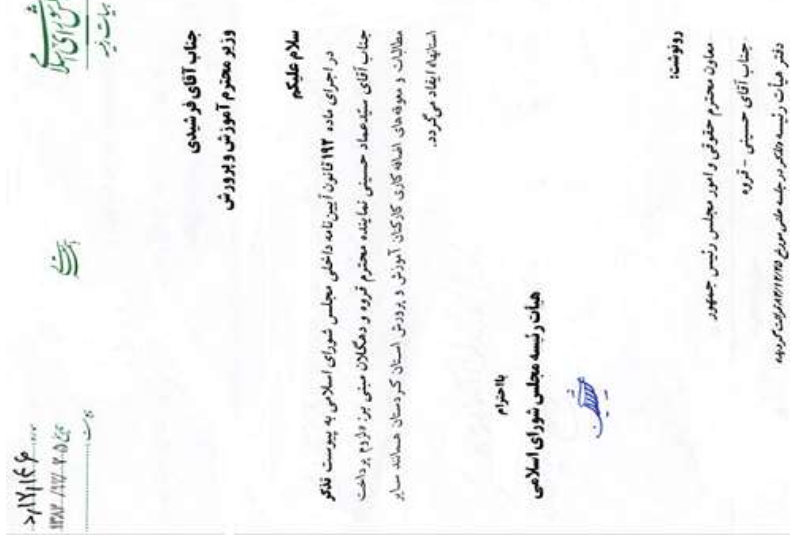
\includegraphics[width=7cm, height=4cm]{letter}


% \section{What is \LaTeX?}
% \LaTeX (usually pronounced ``LAY teck,'' sometimes ``LAH teck,'' and never ``LAY tex'') is a mathematics typesetting program that is the standard for most professional mathematics writing. It is based on the typesetting program \TeX\ created by Donald Knuth of Stanford University (his first version appeared in 1978). Leslie Lamport was responsible for creating \LaTeX\, a more user friendly version of \TeX. A team of \LaTeX\ programmers created the current version,  \LaTeX\ 2$\varepsilon$.

% \section{Math vs. text vs. functions}
% In properly typeset mathematics  variables appear in italics (e.g., $f(x)=x^{2}+2x-3$). The exception to this rule is predefined functions (e.g., $\sin (x)$). Thus it is important to \textbf{always} treat text, variables, and functions correctly. See the difference between $x$ and x, -1 and $-1$, and $sin(x)$ and $\sin(x)$.  

% There are two ways to present a mathematical expression--- \emph{inline} or as an \emph{equation}.

% \subsection{Inline mathematical expressions}
% Inline expressions occur in the middle of a sentence.  To produce an inline expression, place the math expression between dollar signs (\verb!$!).  For example, typing \verb!$90^{\circ}$ is the same as $\frac{\pi}{2}$ radians!  yields $90^{\circ}$ is the same as $\frac{\pi}{2}$ radians.

% \subsection{Equations}
% Equations are mathematical expressions that are given their own line and are centered on the page.  These are usually used for important equations that deserve to be showcased on their own line or for large equations that cannot fit inline. To produce an inline expression, place the mathematical expression  between the symbols  \verb!\[! and \verb!\]!. Typing \verb!\[x=\frac{-b\pm\sqrt{b^2-4ac}}{2a}\]! yields \[x=\frac{-b\pm\sqrt{b^2-4ac}}{2a}.\]
 
% \subsection{Displaystyle} 
% To get full-sized inline mathematical expressions  use  \verb!\displaystyle!. Use this sparingly. Typing \verb!I want this $\displaystyle \sum_{n=1}^{\infty}! \verb!\frac{1}{n}$, not this $\sum_{n=1}^{\infty}! \verb!\frac{1}{n}$.! yields\\ I want  this $\displaystyle \sum_{n=1}^{\infty}\frac{1}{n}$, not this $\sum_{n=1}^{\infty}\frac{1}{n}.$


% \section{Images}

% You can put images (pdf, png, jpg, or gif) in your document. They need to be in the same location as your .tex file when you compile the document. Omit   \verb![width=.5in]! if you want the image to be full-sized.

% \verb!\begin{figure}[ht]!\\
% \verb!\includegraphics[width=.5in]{imagename.jpg}!\\
% \verb!\caption{The (optional) caption goes here.}!\\
% \verb!\end{figure}!

% \subsection{Text decorations}

% Your text can be \textit{italics} (\verb!\textit{italics}!), \textbf{boldface} (\verb!\textbf{boldface}!), or \underline{underlined} (\verb!\underline{underlined}!).

% Your math can contain boldface, $\mathbf{R}$ (\verb!\mathbf{R}!), or blackboard bold, $\mathbb{R}$ (\verb!\mathbb{R}!). You may want to used these to express the sets of real numbers ($\mathbb{R}$ or $\mathbf{R}$), integers ($\mathbb{Z}$ or $\mathbf{Z}$), rational numbers ($\mathbb{Q}$ or $\mathbf{Q}$), and natural numbers ($\mathbb{N}$ or $\mathbf{N}$).

% To have text appear in a math expression use \verb!\text!. \verb!(0,1]=\{x\in\mathbb{R}:x>0\text{ and }x\le 1\}! yields $(0,1]=\{x\in\mathbb{R}:x>0\text{ and }x\le 1\}$. (Without the \verb!\text! command it treats ``and'' as three variables: $(0,1]=\{x\in\mathbb{R}:x>0 and x\le 1\}$.)



% \section{Spaces and new lines}

% \LaTeX\ ignores extra spaces and new lines. For example, 

% \verb!This   sentence will       look!

% \verb!fine after      it is     compiled.!

% This   sentence will       look
% fine after      it is     compiled.


% Leave one full empty line between two paragraphs. Place \verb!\\! at the end of a line to create a new line (but not create a new paragraph).

% \verb!This!

% \verb!compiles!

% ~

% \verb!like\\!

% \verb!this.!

% This
% compiles 

% like\\
% this.

% Use  \verb!\noindent! to prevent a paragraph from indenting.

% \section{Comments}

% Use \verb!%! to create a comment. Nothing on the line after the \verb!%! will be typeset. \verb!$f(x)=\sin(x)$ %this is the sine function! yields $f(x)=\sin(x)$%this is the sine function

% \section{Delimiters}

% \begin{tabular}{lll}
% \emph{description} & \emph{command} & \emph{output}\\
% parentheses &\verb!(x)! & (x)\\
% brackets &\verb![x]! & [x]\\
% curly braces& \verb!\{x\}! & \{x\}\\
% \end{tabular}

% To make your delimiters large enough to fit the content, use them together with \verb!\right! and \verb!\left!. For example, \verb!\left\{\sin\left(\frac{1}{n}\right)\right\}_{n}^! \verb!{\infty}! produces\\ $\displaystyle \left\{\sin\left(\frac{1}{n}\right)\right\}_{n}^{\infty}$.

% Curly braces are non-printing characters that are used to gather text that has more than one character. Observe the differences between the four expressions \verb!x^2!, \verb!x^{2}!, \verb!x^2t!, \verb!x^{2t}! when typeset: $x^2$, $x^{2}$, $x^2t$, $x^{2t}$.


% \section{Lists}

% You can produce ordered and unordered lists.

% \begin{tabular}{lll}
% \emph{description} & \emph{command} & \emph{output}\\
% unordered list&
% \begin{tabular}{l}
% \verb!\begin{itemize}!\\
% \verb!  \item!\\
% \verb!  Thing 1!\\
% \verb!  \item!\\
% \verb!  Thing 2!\\
% \verb!\end{itemize}!
% \end{tabular}&
% \begin{tabular}{l}
% $\bullet$ Thing 1\\
% $\bullet$ Thing 2
% \end{tabular}\\
% ~\\
% ordered list&
% \begin{tabular}{l}
% \verb!\begin{enumerate}!\\
% \verb!  \item!\\
% \verb!  Thing 1!\\
% \verb!  \item!\\
% \verb!  Thing 2!\\
% \verb!\end{enumerate}!
% \end{tabular}&
% \begin{tabular}{l}
% 1.~Thing 1\\
% 2.~Thing 2
% \end{tabular}
% \end{tabular}


% \section{Symbols (in \emph{math} mode)}

% \subsection{The basics}
% \begin{tabular}{lll}
% \emph{description} & \emph{command} & \emph{output}\\
% addition & \verb!+! & $+$\\
% subtraction & \verb!-! & $-$\\
% plus or minus & \verb!\pm! & $\pm$\\
% multiplication (times) & \verb!\times! & $\times$\\
% multiplication (dot) & \verb!\cdot! & $\cdot$\\
% division symbol & \verb!\div! & $\div$\\
% division (slash) & \verb!/! & $/$\\
% circle plus & \verb!\oplus! & $\oplus$\\
% circle times & \verb!\otimes! & $\otimes$\\
% equal & \verb!=! & $=$\\
% not equal & \verb!\ne! & $\ne$\\
% less than & \verb!<! & $<$\\
% greater than & \verb!>! & $>$\\
% less than or equal to & \verb!\le! & $\le$\\
% greater than or equal to & \verb!\ge! & $\ge$\\
% approximately equal to & \verb!\approx! & $\approx$\\
% infinity & \verb!\infty! & $\infty$\\
% dots & \verb!1,2,3,\ldots! & $1,2,3,\ldots$\\
% dots & \verb!1+2+3+\cdots! & $1+2+3+\cdots$\\
% fraction & \verb!\frac{a}{b}! & $\frac{a}{b}$\\
% square root & \verb!\sqrt{x}! & $\sqrt{x}$\\
% $n$th root & \verb!\sqrt[n]{x}! & $\sqrt[n]{x}$\\
% exponentiation & \verb!a^b! & $a^{b}$\\
% subscript & \verb!a_b! & $a_{b}$\\
% absolute value & \verb!|x|! & $|x|$\\
% natural log  & \verb!\ln(x)! & $\ln(x)$\\
% logarithms & \verb!\log_{a}b! & $\log_{a}b$\\
% exponential function & \verb!e^x=\exp(x)! & $e^{x}=\exp(x)$\\
% degree & \verb!\deg(f)! & $\deg(f)$\\
% \end{tabular}
% \newpage

% \subsection{Functions}
% \begin{tabular}{lll}
% \emph{description} & \emph{command} & \emph{output}\\
% maps to & \verb!\to! & $\to$\\
% composition& \verb!\circ! & $\circ$\\
% piecewise& \verb!|x|=! & \multirow{5}{*}{$\displaystyle |x|=\begin{cases}x&x\ge 0\\-x&x<0\end{cases}$}\\
% function&\verb!\begin{cases}!&\\ 
% &\verb!x & x\ge 0\\!&\\ 
% &\verb!-x & x<0!&\\ 
% &\verb!\end{cases}!&
% \end{tabular}

% \subsection{Greek and Hebrew letters}
% \begin{tabular}{llll}
% \emph{command} & \emph{output}&\emph{command} & \emph{output}\\
% \verb!\alpha! & $\alpha$&\verb!\tau! & $\tau$\\
% \verb!\beta! & $\beta$&\verb!\theta! & $\theta$\\
% \verb!\chi! & $\chi$&\verb!\upsilon! & $\upsilon$\\
% \verb!\delta! & $\delta$&\verb!\xi! & $\xi$\\
% \verb!\epsilon! & $\epsilon$&\verb!\zeta! & $\zeta$\\
% \verb!\varepsilon! & $\varepsilon$&\verb!\Delta! & $\Delta$\\
% \verb!\eta! & $\eta$&\verb!\Gamma! & $\Gamma$\\
% \verb!\gamma! & $\gamma$&\verb!\Lambda! & $\Lambda$\\
% \verb!\iota! & $\iota$&\verb!\Omega! & $\Omega$\\
% \verb!\kappa! & $\kappa$&\verb!\Phi! & $\Phi$\\
% \verb!\lambda! & $\lambda$&\verb!\Pi! & $\Pi$\\
% \verb!\mu! & $\mu$&\verb!\Psi! & $\Psi$\\
% \verb!\nu! & $\nu$&\verb!\Sigma! & $\Sigma$\\
% \verb!\omega! & $\omega$&\verb!\Theta! & $\Theta$\\
% \verb!\phi! & $\phi$&\verb!\Upsilon! & $\Upsilon$\\
% \verb!\varphi! & $\varphi$&\verb!\Xi! & $\Xi$\\
% \verb!\pi! & $\pi$&\verb!\aleph! & $\aleph$\\
% \verb!\psi! & $\psi$&\verb!\beth! & $\beth$\\
% \verb!\rho! & $\rho$&\verb!\daleth! & $\daleth$\\
% \verb!\sigma! & $\sigma$&\verb!\gimel! & $\gimel$
% \end{tabular}


% \subsection{Set theory}
% \begin{tabular}{lll}
% \emph{description} & \emph{command} & \emph{output}\\
% set brackets & \verb!\{1,2,3\}! & $\{1,2,3\}$\\
% element of & \verb!\in! & $\in$\\
% not an element of & \verb!\not\in! & $\not\in$\\
% subset of & \verb!\subset! & $\subset$\\
% subset of & \verb!\subseteq! & $\subseteq$\\
% not a subset of & \verb!\not\subset! & $\not\subset$\\
% contains & \verb!\supset! & $\supset$\\
% contains & \verb!\supseteq! & $\supseteq$\\
% union & \verb!\cup! & $\cup$\\
% intersection & \verb!\cap! & $\cap$\\
% big union & 
% \verb!\bigcup_{n=1}^{10}A_n! &
% $\displaystyle \bigcup_{n=1}^{10}A_{n}$\\
% big intersection & \verb!\bigcap_{n=1}^{10}A_n! &$\displaystyle \bigcap_{n=1}^{10}A_{n}$\\
% empty set & \verb!\emptyset! & $\emptyset$\\
% power set & \verb!\mathcal{P}! & $\mathcal{P}$\\
% minimum & \verb!\min! & $\min$\\
% maximum & \verb!\max! & $\max$\\
% supremum & \verb!\sup! & $\sup$\\
% infimum & \verb!\inf! & $\inf$\\
% limit superior & \verb!\limsup! & $\limsup$\\
% limit inferior & \verb!\liminf! & $\liminf$\\
% closure & \verb!\overline{A}! & $\overline{A}$
% \end{tabular}

% \subsection{Calculus}
% \begin{tabular}{lll}
% \emph{description} & \emph{command} & \emph{output}\\
% derivative & \verb!\frac{df}{dx}! & $\displaystyle \frac{df}{dx}$\\
% derivative & \verb!\f'! & $f'$\\
% partial derivative & 
% \begin{tabular}{l}
% \verb!\frac{\partial f}!\\ \verb!{\partial x}! 
% \end{tabular}& $\displaystyle \frac{\partial f}{\partial x}$\\
% integral & \verb!\int! & $\displaystyle\int$\\
% double integral & \verb!\iint! & $\displaystyle\iint$\\
% triple integral & \verb!\iiint! & $\displaystyle\iiint$\\
% limits & \verb!\lim_{x\to \infty}! & $\displaystyle \lim_{x\to \infty}$\\
% summation  & 
% \verb!\sum_{n=1}^{\infty}a_n! &
% $\displaystyle \sum_{n=1}^{\infty}a_n$\\
% product  & 
% \verb!\prod_{n=1}^{\infty}a_n! &
% $\displaystyle \prod_{n=1}^{\infty}a_n$
% \end{tabular}




% \subsection{Logic}
% \begin{tabular}{lll}
% \emph{description} & \emph{command} & \emph{output}\\
% not & \verb!\sim! & $\sim$\\
% and & \verb!\land! & $\land$\\
% or & \verb!\lor! & $\lor$\\
% if...then & \verb!\to! & $\to$\\
% if and only if & \verb!\leftrightarrow! & $\leftrightarrow$\\
% logical equivalence & \verb!\equiv! & $\equiv$\\
% therefore & \verb!\therefore! & $\therefore$\\
% there exists  & \verb!\exists! & $\exists$\\
% for all & \verb!\forall! & $\forall$\\
% implies & \verb!\Rightarrow! & $\Rightarrow$\\
% equivalent & \verb!\Leftrightarrow! & $\Leftrightarrow$
% \end{tabular}

% \subsection{Linear algebra}
% \begin{tabular}{lll}
% \emph{description} & \emph{command} & \emph{output}\\
% vector & \verb!\vec{v}! & $\vec{v}$\\
% vector & \verb!\mathbf{v}! & $\mathbf{v}$\\
% norm & \verb!||\vec{v}||! & $||\vec{v}||$\\
% matrix&
% \begin{tabular}{l}
% \verb!\left[!\\
% \verb!\begin{array}{ccc}!\\
% \verb!1 & 2 & 3 \\!\\
% \verb!4 & 5 & 6\\!\\
% \verb!7 & 8 & 0!\\
% \verb!\end{array}!\\
% \verb!\right]!\end{tabular}&
% $\displaystyle \left[\begin{array}{ccc}1 & 2 & 3 \\4 & 5 & 6 \\7 & 8 & 0\end{array}\right]$\\
% \\determinant&
% \begin{tabular}{l}
% \verb!\left|!\\
% \verb!\begin{array}{ccc}!\\
% \verb!1 & 2 & 3 \\!\\
% \verb!4 & 5 & 6 \\!\\
% \verb!7 & 8 & 0!\\
% \verb!\end{array}!\\
% \verb!\right|!
% \end{tabular}&
% $\displaystyle \left|\begin{array}{ccc}1 & 2 & 3 \\4 & 5 & 6 \\7 & 8 & 0\end{array}\right|$\\
% determinant & \verb!\det(A)! & $ \det(A)$\\
% trace & \verb!\operatorname{tr}(A)! & $\operatorname{tr}(A)$\\
% dimension & \verb!\dim(V)! & $\dim(V)$\\
% \end{tabular}

% \subsection{Number theory}
% \begin{tabular}{lll}
% \emph{description} & \emph{command} & \emph{output}\\
% divides & \verb!|! & $|$\\
% does not divide & \verb!\not |! & $\not |$\\
% div & \verb!\operatorname{div}! & $\operatorname{div}$\\
% mod & \verb!\mod! & $\operatorname{mod}$\\
% greatest common divisor & \verb!\gcd! & $\gcd$\\
% ceiling & \verb!\lceil x \rceil! & $\lceil x\rceil$\\
% floor & \verb!\lfloor x \rfloor! & $\lfloor x \rfloor$\\
% \end{tabular}




% \subsection{Geometry and trigonometry}
% \begin{tabular}{lll}
% \emph{description} & \emph{command} & \emph{output}\\
% angle& \verb!\angle ABC! & $\angle ABC$\\
% degree& \verb!90^{\circ}! & $90^{\circ}$\\
% triangle& \verb!\triangle ABC! & $\triangle ABC$\\
% segment& \verb!\overline{AB}! & $\overline{AB}$\\
% sine& \verb!\sin! & $\sin$\\
% cosine& \verb!\cos! & $\cos$\\
% tangent& \verb!\tan! & $\tan$\\
% cotangent& \verb!\cot! & $\cot$\\
% secant& \verb!\sec! & $\sec$\\
% cosecant& \verb!\csc! & $\csc$\\
% inverse sine& \verb!\arcsin! & $\arcsin$\\
% inverse cosine& \verb!\arccos! & $\arccos$\\
% inverse tangent& \verb!\arctan! & $\arctan$\\
% \end{tabular}

% \section{Symbols (in \emph{text} mode)}

% The followign symbols do \textbf{not} have to be surrounded by dollar signs.

% \begin{tabular}{lll}
% \emph{description} & \emph{command} & \emph{output}\\
% dollar sign & \verb!\$! & \$ \\
% percent & \verb!\%! & \% \\
% ampersand & \verb!\&! & \& \\
% pound & \verb!\#! & \# \\
% backslash & \verb!\textbackslash! & \textbackslash \\
% left quote marks & \verb!``! & `` \\
% right quote marks & \verb!''! & '' \\
% single left quote  & \verb!`! & ` \\
% single right quote  & \verb!'! & ' \\
% hyphen & \verb!X-ray! & X-ray\\
% en-dash & \verb!pp. 5--15! & pp. 5--15 \\
% em-dash & \verb!Yes---or no?! & Yes---or no? 
% \end{tabular}

% \section{Resources}
% Great symbol look-up site: \href{http://detexify.kirelabs.org/}{Detexify}\\
% \href{http://amath.colorado.edu/documentation/LaTeX/Symbols.pdf}{\LaTeX\ Mathematical Symbols}\\
% \href{ftp://tug.ctan.org/pub/tex-archive/info/symbols/comprehensive/symbols-letter.pdf}{The Comprehensive \LaTeX\ Symbol List}\\ 
% \href{http://mirrors.med.harvard.edu/ctan/info/lshort/english/lshort.pdf}{The Not So Short Introduction to \LaTeX\ 2$\varepsilon$}\\
% \href{http://www.tug.org/}{TUG: The \TeX\ Users Group}\\
% \href{http://www.ctan.org/}{CTAN: The Comprehensive \TeX\ Archive Network}\\
% ~\\
% \LaTeX\ for the Mac: \href{http://www.tug.org/mactex/}{Mac\TeX}\\
% \LaTeX\ for the PC: \href{http://www.texniccenter.org/}{{\TeX}nicCenter} and \href{http://miktex.org/}{MiK\TeX}\\
% \LaTeX\ online: \href{http://www.writelatex.com/}{WriteLaTeX}.
% \vfill
% \hrule
% ~\\
% Dave Richeson, Dickinson College, \href{http://divisbyzero.com/}{http://divisbyzero.com/}
\end{multicols*}

\end{document}
